\documentclass[12pt,a4paper]{article}
%-- coding: UTF-8 --
\usepackage[UTF8]{ctex}
\usepackage[utf8]{inputenc}
\usepackage{geometry}
\usepackage{graphicx} % 引入图片
\usepackage{enumitem} % 取消列表默认间距
\geometry{left=3.18cm,right=3.18cm,top=2.54cm,bottom=2.54cm}
\usepackage{hyperref}
\hypersetup{hidelinks,
	colorlinks=true,
	allcolors=black,
	pdfstartview=Fit,
	breaklinks=true}
\usepackage{listings}
\usepackage{xcolor}
\usepackage{fontspec}
\usepackage{booktabs} % 三线表

\usepackage{tikz}
\usepackage{amsmath}
\usepackage{colortbl}
\newcommand\y{\cellcolor{clight2}}
\definecolor{clight2}{RGB}{212, 237, 244}%
\newcommand\tikznode[3][]%
   {\tikz[remember picture,baseline=(#2.base)]
      \node[minimum size=0pt,inner sep=0pt,#1](#2){#3};%
   }
\tikzset{>=stealth}
\renewcommand\vec[1]{\mathbf{#1}}

% 嵌入代码风格
\lstset{
	language    = c++,
	breaklines  = true,
	captionpos  = b,
	tabsize     = 4,
	columns     = fullflexible,
	commentstyle = \color[RGB]{0,128,0},
	keywordstyle = \color[RGB]{0,0,255},
	basicstyle   = \small\ttfamily,
	stringstyle  = \color[RGB]{148,0,209}\ttfamily,
	rulesepcolor = \color{red!20!green!20!blue!20},
	showstringspaces = false,
}



\title{实验二 \hspace{0.5cm} 树与分治策略}
\author{}
\date{October, 2024}

\begin{document}
\maketitle

\section{前言}

\textbf{分治(divide and conquer)},字面上的解释是“分而治之”,就是把一个复杂的问题分解成两个或多个相同或相似的\textbf{子问题},再把子问题分成更小的子问题,直到子问题的规模足够简单可以直接求解。在计算机科学汇总,分治法是很多高效算法的基础,如排序算法(快速排序,归并排序),傅里叶变换(快速傅里叶变换)等等。分治法在实际问题中具有很高的指导意义,例如全国人口普查过程中,可以将问题递归地拆分成省级、市级、区级、乡镇级、街道级、小区级,自下而上的统计人数。分治法的主要实现步骤如下:
\begin{enumerate}[noitemsep]
    \item 分治(Divide):将原问题分解为若干个规模较小,相互独立,与原问题形式相同的子问题。
    \item 解决(Conquer):若当前问题规模足够小,直接返回答案,否则递归地解决每个子问题。
    \item 合并(Combine):将各个问题的解合并为原问题的解。
\end{enumerate}

如果题目符合下面性质,或许可以用分治法来解决:
\begin{enumerate}[noitemsep]
    \item 该问题的规模缩小到一定程度就可以容易的解决。
    \item 该问题可以分解为若干个规模较小的相同问题,即该问题具有最优子结构性质。
    \item 利用该问题分解出的子问题的解可以合并为该问题的解。
\end{enumerate}

\textbf{递归(recursion)} 是分治中非常重要的步骤,在数学和计算机科学中,递归是指在函数调用函数本身。递归一词常用于描述以自身相似方法重复事物的过程。例如,当两面镜子相互之间近似平行时,镜中嵌套的图像是以无限递归的形式出现的。将时光往前推,在中国还流传着这样一个有趣的故事:从前有座山,山里有座庙,庙里有个老和尚,正在给小和尚讲故事呢!故事是什么呢?“从前有座山,山里有座庙,庙里有个老和尚,正在给小和尚讲故事呢!故事是什么呢?'从前有座山,山里有座庙,庙里有个老和尚,正在给小和尚讲故事呢!故事是什么呢?'”

上面的故事似乎是没有终点的,如果将故事写成计算机程序然后运行,恐怕不到一会程序就会崩溃,因为递归调用函数会在系统栈中维护函数栈,无限递归下去会使得系统栈超出内存。图1所示的图形被称为\textbf{德罗斯特效应}(Droste effect),是递归的一种视觉形式,是指一张照片的某个部分与整张图片相同,如此产生无限循环。这张照片是通过名为 Mathmp 的数学软件制作出来的,使用 PhotoShop 的 Droste Effect 滤镜也可以制作出这种效果。

在计算机程序中,递归实现并不是任何一个算法必须要有的部分。理论上,任何的递归都可以使用分支语句和循环语句实现,只不过不使用递归的实现难度远远超过了递归实现。因此,有效的利用递归可以帮助我们更轻松的解决实际问题。本节实验课的基本内容是两个非常经典的题目,它们都可以优雅地使用分治法进行分析,并使用递归来求解。


\begin{figure}
    \centering
    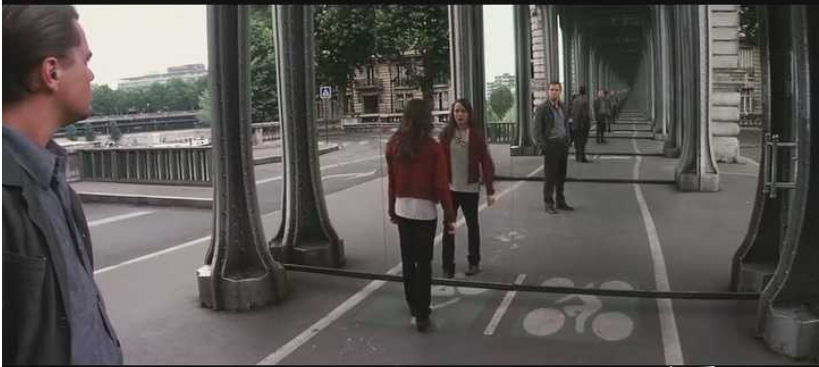
\includegraphics[width=10cm]{img/lab2/drosteeffect.png}
    \caption{《盗梦空间》(Inception,2010)中带有“德罗斯特效应”性质的电影镜头。}
    \label{fig:my_label}
\end{figure}


\section{实验项目结构}

\begin{itemize}[noitemsep]
    \item[$-$] find\_maximum\_subarray
        \begin{itemize}[noitemsep]
            \item[$-$] include
                \begin{itemize}[noitemsep]
                    \item[$\bullet$] util.hpp
                    \item[$\bullet$] Solution.hpp
                \end{itemize}
            \item[$-$] data
            \item[$\bullet$] main.cpp
        \end{itemize}
    \item[$-$] round\_robin\_schedule
        \begin{itemize}[noitemsep]
            \item[$-$] 略
        \end{itemize}
    \item[$-$] perfect\_permutation
        \begin{itemize}
            \item[$-$] 略
        \end{itemize}
\end{itemize}

\textbf{本实验包含三个独立的题目:find\_maximum\_subarray(最大子序列) 和 round\_robin\_schedule(循环赛时间表),perfect\_permutation(拓展题:完美排列)}。

每个题目的代码结构是类似的,include 文件夹中包含了 \textcolor{blue}{util.hpp(包含测试用及一些常量和工具包的引入,请不要对其进行任何修改)} 和 \textcolor{blue}{Solution.hpp(你唯一需要写的文件)},data 文件夹中包含了测试数据,对于每个题目,你需要完成\textbf{该题目的 Solution.hpp }的编写,然后编译运行\textbf{该题目的 main.cpp }来进行校验,校验通过后请将代码\textbf{提交到OJ上}。

\textcolor{red}{请注意,每次对 Solution.hpp 修改完之后,需要重新编译运行\textbf{相应题目的 main.cpp},如果直接执行上次编译好的 main.exe 或 main,新的修改将不会生效。}




\section{实验内容}

\subsection{最大子序列}

给定一个长度为 $N$ 的数组 $A$,其任意连续子序列可以表示为 $A_i, A_{i+1}, \cdots, A_{j}$,其中 $0\le i \le j \le N-1$。最大子序列是指所有的子序列中和最大的那一个,注意子序列不能为空。为了降低难度,你需要输出它的和,即:
$$result = \max_{0\le i\le j \le N-1}{\sum_{k=i}^j A[k]}$$

例如:[-2, 11, -4, 13, -5, -2] 的答案为 20。

请\textcolor{red}{根据课件中的伪代码}思想完成 Solution.hpp 的实现。

\begin{lstlisting}
    class Solution {
    public:
        int find_maximum_crossing_subarray(vector<int> &A, int low, int mid, int high) {
            // 请在这里完成你的代码
            return 0
        }
        int find_maximum_subarray(vector<int> &A, int low, int high) {
            // 请在这里完成你的代码
            return 0
        }
        int find_maximum_subarray(vector<int> &A) {
            return find_maximum_subarray(A, 0, A.size() - 1);
        }
    };
\end{lstlisting}

测试数据范围:$N\le 10^5$, $|A[i]| \le 10000$。



\subsection{循环赛日程表}

设有 $n=2^k$ 个运动员要进行羽毛球循环赛,现要设计一个满足以下要求的比赛日程表:

\begin{itemize}[noitemsep]
    \item 每个选手必须与其他 $n-1$ 个选手各比赛一次
    \item 每个选手一天只能比赛一次
    \item 循环赛一共需要进行 $n-1$ 天
\end{itemize}

一些例子:

\begin{itemize}
    \item n = 2 时的日程表如下表所示:\\ \\
          \begin{tabular}{cc}
              \toprule
              运动员 & 第一天 \\
              \midrule
              1   & 2   \\
              2   & 1   \\
              \bottomrule
          \end{tabular} \\

    \item n = 4 时的日程表如下表所示:

          \begin{tabular}{cccc}
              \toprule
              运动员 & 第一天 & 第二天 & 第三天 \\
              \midrule
              1   & 2   & 3   & 4   \\
              2   & 1   & 4   & 3   \\
              3   & 4   & 1   & 2   \\
              4   & 3   & 2   & 1   \\
              \bottomrule
          \end{tabular} \\

    \item n = 8 时的日程表如下表所示:

          \begin{tabular}{cccccccc}
              \toprule
              运动员 & 第一天 & 第二天 & 第三天 & 第四天 & 第五天 & 第六天 & 第七天 \\
              \midrule
              1   & 2   & 3   & 4   & 5   & 6   & 7   & 8   \\
              2   & 1   & 4   & 3   & 6   & 5   & 8   & 7   \\
              3   & 4   & 1   & 2   & 7   & 8   & 5   & 6   \\
              4   & 3   & 2   & 1   & 8   & 7   & 6   & 5   \\
              5   & 6   & 7   & 8   & 1   & 2   & 3   & 4   \\
              6   & 5   & 8   & 7   & 2   & 1   & 4   & 3   \\
              7   & 8   & 5   & 6   & 3   & 4   & 1   & 2   \\
              8   & 7   & 6   & 5   & 4   & 3   & 2   & 1   \\
              \bottomrule
          \end{tabular}

\end{itemize}


你需要实现 Solution 类中的 round\_robin\_schedule 方法,对于传入的参数 $n$,返回一个大小为 $n\times n$ 的二维数组。该二维数组满足:
\begin{itemize}[noitemsep]
    \item 所有元素都在 $[1, n]$ 范围内。
    \item 第一列从上到下依次为 $1\sim n$。
    \item 同行或同列的元素不能相同。
\end{itemize}


\begin{lstlisting}
    class Solution {
    public:
        vector<vector<int>> round_robin_schedule(int n) {
            // 如此构造一个二维数组( nxn 矩阵)
            // ans[i][j]表示矩阵的第i行第j列
            vector<vector<int> > ans;
            for(int i=0; i<n; i++) {
            ans.push_back(vector<int>(n, 0));
            }
            // 请在这里完成你的代码
            return ans;
        }
    };
\end{lstlisting}

\textbf{提示:} 按照分治策略,将所有选手分成两部分。令$m=n/2$,当得到了 m 名选手前 m 天的日程表后(左上角 $m\times m$ 矩阵),通过平移、交换等方式分别拼凑出后m名选手前 m 天的日程表和 n 名选手后 m 天的日程表。下面的示意图中,$n=4, m=2$。

\begin{figure}[h]
    \centering
    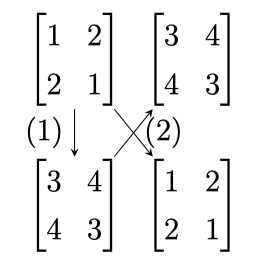
\includegraphics[width=3.5cm]{img/lab2/tips2.png}
\end{figure}

在具体实现过程中,你可以使用 vector 的 resize() 方法来调整数组大小。

测试数据范围:$1 \le k \le 10, n = 2^k$。


\section{实验思考}
\begin{enumerate}
    \item 对于序列 [3, 2, -5, 3, -9, 9, -4, 6],画出求解最大子序列的递归调用树,并标出每个函数的返回值。
    \item 分析两个实验的时空复杂度。
    \item 如果最大子序列问题中允许选择空的子序列(和为 0 ),代码应该如何修改?

    \item 【拓展题】完美排列(Google 面试题)\\
          如果一个长度为 $n(1 \le n \le 10^3)$ 的排列 $a$ 满足对于每对 $i, j(i<j)$,都不存在 $k(i < k < j)$ 使得 $a[k]*2 = a[i] + a[j]$ 成立,那么该排列就被称为完美排列。给定 $n$,请你求出任意一个长度为 $n$ 的完美排列。\\
          注意:长度为 $n$ 的排列是指由整数 $1,2,\cdots, n$ 构成的数组。\\
          例如,n = 4 时,完美排列可以是 [1,3,2,4], n = 5 时,完美排列可以是 [1,5,3,2,4], n = 9 时,完美排列可以是 [1,9,5,3,7,2,6,4,8]。\\
          \textbf{提示:} 分奇偶考虑

    \item 【扩展题】快速幂\\
          计算$a$的$n$次方表示将$n$个$a$乘在一起:$a^n=\underbrace{a\times a\dots \times a}_{n\mbox{个}a}$,暴力的计算需要$O(n)$的时间,请考虑如何使用分治思想加速这个计算过程($a,n$均为非负整数)。\\
          由于数值可能过大,返回对一个给定的正整数$p$取模后的结果。
          \begin{itemize}
              \item input \\ $a$ $b$ $p$ (其中$1 \le a, b, p \le 10^9$)
              \item output \\ $a^b$ mod $p$
              \item 提示:注意 int 乘法可能会溢出,需要使用 long long。
          \end{itemize}
    \item 【补充】快速傅里叶变换(感兴趣的同学可以自行了解,不做要求) \\
          大家在高数中都学习到过傅里叶变换(Fourier Transform),由于计算机无法处理无限连续域,为了便于计算机处理,出现了离散傅里叶变换(Discrete Fourier Transform)。快速傅里叶变换就是将离散傅里叶变换与分治思想相结合的产物,其典型应用是加速计算两个n度多项式的乘法。
          \begin{itemize}
              \item 例如对于两个多项式 $A=5x^2+3x+7,B=7x^2+2x+1$,两个多项式的乘积$C=A\times B=35x^4+31x^3+60x^2+17x+7$,我们可以在$O(n^2)$的时间复杂度中解得。而快速傅里叶变换可以将这个复杂度降低至$O(nlogn)$。
              \item 由于大整数也可以表示为多项式的形式(如$123=1\times 10^2+2\times 10^1+3\times 10^0$),因此快速傅里叶变换还可以用来加速大整数的乘法,类似的还有许多其他应用场景。
          \end{itemize}

\end{enumerate}


\section{其他}

\subsection{vector 的基本使用}

vector 可以被简单的看做是一个动态数组,可以像普通的数组一样使用 $[]$ 运算符来访问其中的元素。与普通数组不同的是,它可以方便的进行创建、调整大小、添加或删除元素等等。
\begin{lstlisting}
    #include <vector> // 引入头文件
    // 1. 定义方法:
    vector<int> a; // 定义一个元素类型为 int 的动态数组 a
    vector<int> b(10); // 定义一个包含 10 个 int(默认为 0) 的动态数组 b
    vector<int> c(10, 100); // 定义一个包含 10 个 100 的动态数组 c
    // 2. 访问元素
    int x = c[0]; // 访问 c 中下标为 0 的元素
    // 3. 获取数组大小
    int n = c.size();
    // 4. 判断数组是否为空
    if(a.empty()) {
        // 为空则 if 条件成立
    }
    // 5. 插入元素
    a.push_back(x); // 把 x 插入到 a 的尾部
    // 6. 删除元素
    a.pop_back(); // 删除 a 的最后一个元素
    // 7. 清空数组
    c.clear();
\end{lstlisting}

有关更多内容,你可以参考:

\begin{itemize}[noitemsep]
    \item \href{https://www.runoob.com/w3cnote/cpp-vector-container-analysis.html}{https://www.runoob.com/w3cnote/cpp-vector-container-analysis.html}
    \item \href{https://en.cppreference.com/w/cpp/container/vector}{https://en.cppreference.com/w/cpp/container/vector}
    \item \href{https://www.w3cschool.cn/cpp/cpp-i6da2pq0.html}{https://www.w3cschool.cn/cpp/cpp-i6da2pq0.html}
    \item \href{http://c.biancheng.net/view/6749.html}{http://c.biancheng.net/view/6749.html}
\end{itemize}


\end{document}